$  $\chapter{Arhitektura i dizajn sustava}
		
		\textbf{\textit{dio 1. revizije}}\\

		\textit{ Potrebno je opisati stil arhitekture te identificirati: podsustave, preslikavanje na radnu platformu, spremišta podataka, mrežne protokole, globalni upravljački tok i sklopovsko-programske zahtjeve. Po točkama razraditi i popratiti odgovarajućim skicama:}
	\begin{itemize}
		\item 	\textit{izbor arhitekture temeljem principa oblikovanja pokazanih na predavanjima (objasniti zašto ste baš odabrali takvu arhitekturu)}
		\item 	\textit{organizaciju sustava s najviše razine apstrakcije (npr. klijent-poslužitelj, baza podataka, datotečni sustav, grafičko sučelje)}
		\item 	\textit{organizaciju aplikacije (npr. slojevi frontend i backend, MVC arhitektura) }		
	\end{itemize}

	
		

		

				
		\section{Baza podataka}
			
		Za naš projekt odabrali smo \textbf{relacijsku bazu podataka} zbog njezine pogodnosti da prikaže mali dio stvarnog svijeta bez redundancije unutar same baze. Dohvaćanje podataka je jako brzo i jako lagano se može paralelizirati. Specifičnu implementaciju relacijske baze podataka koju smo odabrali je \textbf{PostgreSQL}. To je open source baza podataka s preko 30 godina aktivnog razvoja zbog kojega je zaslužila svoju čvrstu reputaciju za pouzdanost, bogatstvo opcijama i visokim performansama. Zbog načina na koji je SQL standard napisan, vrlo je slična ostalim SQL bazama podataka.\\ 
		
		Tijekom razvoja koristimo \textbf{H2 bazu}. To je privremena baza podataka koja služi za testiranje koda. Svi zapisi u njoj se nalaze u privremenoj memoriji i nisu perzistentni. Zbog toga je odlična za testiranje. Ona je open source, napisana u Javi i ima čvrste sigurnosne postavke. Na nju se isto može povezati s više konekcija i baza podataka je enkriptirana SHA-256 enkripcijom. Ima vrlo malu potrošnju memorije i jako malo mjesta zauzima na disku (oko 2MB). \\ 
		
		Također koristimo \textbf{JPA (Java Persistence API)} koje samo sadrži sučelja za stvaranje Persistence layouta. Dopušta nam da mapiramo entitete tablica i veze između tablica na objekte u Javi. Ovo sučelje definira svoj vlastiti query jezik (JPQA). JPQA prevoditelj interpretira kod i piše SQL queryje. JPA ne možemo samostalno koristiti, već nam treba konkretna implementacija toga sučelja. Implementaciju koju ćemo mi koristiti se zove Hibernate. \\ 
		
		Na bazu podataka se iz Jave spajamo preko \textbf{JdbcTemplatea}. To je snažni mehanizam za spajanje i izvođenje SQL queryja. On nam smanjuje količinu koda koju moramo napisati kako bismo izvršavali queryje, kao što je spajanje na bazu, kreiranje izraza i zatvaranje spoja. \\
		
	Naša baza podataka sastoji se od sljedećih tablica:
		\begin{itemize}[noitemsep]
		\item
			user
		\item
			friends
		\item
			friendship-req
		\item
			role
		\item
			event
		\item
			event-attendance
		\item
			event-path
		\item
			path
		\item
			badge
		\item
			user-badge
		\item
			notification
		\item
			hill
		\item
			mountain-lodge
		\item
			utility
		\item
			lodge-utility
		\item
			path-user-grade
		\item
			path-wishlist
		\item
			completed-paths
		\item
			report-path
		\item
			visit-confirmation-request
		\item
			mountaneer-on-duty
		\item
			place-of-residence	


\end{itemize}
		
		\definecolor{LightBlue}{rgb}{0.67, 0.9, 0.93}
		\definecolor{LightGreen}{rgb}{0.4, 1.0, 0.0}
		
			\subsection{Opis tablica}
			Primarni ključevi su označeni žutom, a strani ključevi plavom bojom.\\
			
%Tablice
			\textbf{user}  Ovaj entitet sadrži sve važne informacije o korisniku aplikacije. Sadrži atribute: name, email, password, image, role-id.  Ova tablica je u Many-to-One vezi s tablicom role preko atributa korisnika role-id.
			
			\begin{longtabu} to \textwidth {|X[6, l]|X[6, l]|X[20, l]|}
				\hline \multicolumn{3}{|c|}{\textbf{user - ime tablice}}	 \\[3pt] \hline
				\endfirsthead
				
				\hline \multicolumn{3}{|c|}{\textbf{user - ime tablice}}	 \\[3pt] \hline
				\endhead
				
				\hline 
				\endlastfoot
				
				\cellcolor{LightBlue} id & INT	&  	jedinstveni identifikator korisnika	\\ \hline
				name	& VARCHAR &  ime i prezime korisnika 	\\ \hline 
				email & VARCHAR &  email korisnika \\ \hline 
				password & VARCHAR	&  	lozinka korisnika	\\ \hline 
				image & bytea	&  	slika korisnika	\\ \hline 
				role-id & FOREIGN-KEY(role-id)	&  	strani ključ uloge korisnika	\\ \hline 
				address & int	&  	adresa stanovanja korisnika	\\ \hline 
				place-id & FOREIGN-KEY(place-of-residence) & strani ključ mjesta stanovanja korisnika \\ \hline
				date-of-birth & date & datum rođenja korisnika \\ \hline
				
				
			\end{longtabu}
			\vspace{10mm}
			
			\textbf{place-of-residence}  Ovaj entitet sadrži informaciju o različitim mjestima stanovanja. Povezuje se s tablicom korisnika.
			
			\begin{longtabu} to \textwidth {|X[6, l]|X[6, l]|X[20, l]|}
				
				\hline \multicolumn{3}{|c|}{\textbf{place-of-residence - ime tablice}}	 \\[3pt] \hline
				\endfirsthead
				
				\hline \multicolumn{3}{|c|}{\textbf{place-of-residence - ime tablice}}	 \\[3pt] \hline
				\endhead
				
				\hline 
				\endlastfoot
				
				\cellcolor{LightGreen}id & INT	&  	jedinstveni identifikator mjesta stanovanja	\\ \hline
				name	& VARCHAR &  ime mjesta stanovanja 	\\ \hline 
				%\cellcolor{LightBlue} primjer	& VARCHAR &   	\\ \hline 
				
				
			\end{longtabu}
			\vspace{10mm}
			
			\textbf{friends} Ovaj entitet sadrži informaciju o Many-To-Many prijateljskoj vezi između dva korisnika. Sadrži atribute: userId1, userId2, koji su oba strani ključevi iz tablice user
			
			\begin{longtabu} to \textwidth {|X[6, l]|X[6, l]|X[20, l]|}
				
				\hline \multicolumn{3}{|c|}{\textbf{friends - ime tablice}}	 \\[3pt] \hline
				\endfirsthead
				
				\hline \multicolumn{3}{|c|}{\textbf{friends - ime tablice}}	 \\[3pt] \hline
				\endhead
				
				\hline 
				\endlastfoot
				
				\cellcolor{LightGreen}userId1 & FOREIGN-KEY(user)	&  strani ključ 1. korisnika	\\ \hline
				userId2	& FOREIGN-KEY(user) &   strani ključ 2. korisnika	\\ \hline 
				created-on	& date &   datum stvaranja prijateljstva	\\ \hline 
				%\cellcolor{LightBlue} primjer	& VARCHAR &   	\\ \hline 
				
				
			\end{longtabu}
			\vspace{10mm}

			\textbf{friendship-req} Ovaj entitet sadrži informaciju o poslanom zahtjevu za prijateljstvo između 2 korisnika. Sadrži atribute: friendship-send, friendship-recieve, koji su oba strani ključevi iz tablice user
			
			\begin{longtabu} to \textwidth {|X[6, l]|X[6, l]|X[20, l]|}
				
					\hline \multicolumn{3}{|c|}{\textbf{friendship-req - ime tablice}}	 \\[3pt] \hline
				\endfirsthead
				
				\hline \multicolumn{3}{|c|}{\textbf{friendship-req - ime tablice}}	 \\[3pt] \hline
				\endhead
				
				\hline 
				\endlastfoot
				
				\cellcolor{LightGreen}friendship-send & FOREIGN-KEY(user)	&  strani ključ korisnika koji šalje zahtjev za prijateljstvom 	\\ \hline
				friendship-recieve	& FOREIGN-KEY(user) &   strani ključ korisnika koji prima zahtjev za prijateljstvom	\\ \hline 
				%\cellcolor{LightBlue} primjer	& VARCHAR &   	\\ \hline 
				
				
			\end{longtabu}
			\vspace{10mm}
		
			\textbf{role} Ovaj entitet sadrži informaciju o ulozi koju ima određeni korisnik. Određuje razinu dozvole korisnika
			
			\begin{longtabu} to \textwidth {|X[6, l]|X[6, l]|X[20, l]|}
				
				\hline \multicolumn{3}{|c|}{\textbf{role - ime tablice}}	 \\[3pt] \hline
				\endfirsthead
				
				\hline \multicolumn{3}{|c|}{\textbf{role - ime tablice}}	 \\[3pt] \hline
				\endhead
				
				\hline 
				\endlastfoot
				
				\cellcolor{LightGreen}id & int	&  jedinstveni ID uloge	\\ \hline
				name	& VARCHAR &  ime uloge 	\\ \hline 
				%\cellcolor{LightBlue} primjer	& VARCHAR &   	\\ \hline 

			\end{longtabu}
			\vspace{10mm}

			\textbf{event} Ovaj entitet sadrži informaciju o događaju. Sadrži atribute: name, description, start-date, end-date, date-created i u One-To-Many je vezi s tablicom user preko atributa author-id.
			
			\begin{longtabu} to \textwidth {|X[6, l]|X[6, l]|X[20, l]|}
				
				\hline \multicolumn{3}{|c|}{\textbf{event - ime tablice}}	 \\[3pt] \hline
				\endfirsthead
				
				\hline \multicolumn{3}{|c|}{\textbf{event - ime tablice}}	 \\[3pt] \hline
				\endhead
				
				\hline 
				\endlastfoot
				
				\cellcolor{LightGreen}id & int	&  	jedinstveni id događaja 	\\ \hline
				name	& VARCHAR & ime događaja  	\\ \hline 
				description & VARCHAR &  opis događaja \\ \hline 
				start-date & timestamp	&  	datum početka događaja	\\ \hline 
				end-date & timestamp	&  	datum kraja događaja	\\ \hline 
				date-created & timestamp	&  	datum stvaranja događaja	\\ \hline 
				author-id & FOREIGN-KEY(user)	& strani ključ korisnika koji je stvorio događaj 		\\ \hline 
				%\cellcolor{LightBlue} primjer	& VARCHAR &   	\\ \hline 
				
				
			\end{longtabu}
			\vspace{10mm}

			\textbf{event-attendance} Ovaj entitet sadrži informaciju o Many-To-Many učestvovanju na nekom događaju nekog korisnika. Sadrži atribute: user-id, event-id koji su oba strani ključevi.
			
			\begin{longtabu} to \textwidth {|X[6, l]|X[6, l]|X[20, l]|}
				
				\hline \multicolumn{3}{|c|}{\textbf{event-attendance - ime tablice}}	 \\[3pt] \hline
				\endfirsthead
				
				\hline \multicolumn{3}{|c|}{\textbf{event-attendance - ime tablice}}	 \\[3pt] \hline
				\endhead
				
				\hline 
				\endlastfoot
				
				\cellcolor{LightGreen}user-id & FOREIGN-KEY(user)	&  	strani ključ korisnika koji će prisustvovati događaju 	\\ \hline
				event-id	& FOREIGN-KEY(user) &  strani ključ događaja kojemu određena osoba pristupa	\\ \hline 
				%\cellcolor{LightBlue} primjer	& VARCHAR &   	\\ \hline 
				
				
			\end{longtabu}
			\vspace{10mm}		
			
			\textbf{event-path} Ovaj entitet sadrži informaciju o Many-To-Many vezi između staze i nekog događaja. Sadrži atribute: path-id, event-id koji su oba strani ključevi.
			
			\begin{longtabu} to \textwidth {|X[6, l]|X[6, l]|X[20, l]|}
				
				\hline \multicolumn{3}{|c|}{\textbf{event-path - ime tablice}}	 \\[3pt] \hline
				\endfirsthead
				
				\hline \multicolumn{3}{|c|}{\textbf{event-path - ime tablice}}	 \\[3pt] \hline
				\endhead
				
				\hline 
				\endlastfoot
				
				\cellcolor{LightGreen}path-id & FOREIGN-KEY(path)	&  	strani ključ staze koja je dio nekog događaja	\\ \hline
				event-id	& FOREIGN-KEY(user) &  strani ključ događaja u kojemu se pojedina staza koristi	\\ \hline 
				%\cellcolor{LightBlue} primjer	& VARCHAR &   	\\ \hline 
				
				
			\end{longtabu}
			\vspace{10mm}

			\textbf{path} Ovaj entitet sadrži informacije o pojedinoj stazi. Sadrži atribute: name, start, end, avg-walk-time, length, sea-level-diff, date-created, is-private, author-id, hill-id
			
			\begin{longtabu} to \textwidth {|X[6, l]|X[6, l]|X[20, l]|}
				
				\hline \multicolumn{3}{|c|}{\textbf{path - ime tablice}}	 \\[3pt] \hline
				\endfirsthead
				
				\hline \multicolumn{3}{|c|}{\textbf{path - ime tablice}}	 \\[3pt] \hline
				\endhead
				
				\hline 
				\endlastfoot
				
				\cellcolor{LightGreen}id & int	&  	jedinstveni ID staze	\\ \hline
				name	& VARCHAR &   ime staze	\\ \hline 
				start & VARCHAR & ime početne staze  \\ \hline 
				end & VARCHAR &  ime završne staze \\ \hline 
				avg-walk-time & time &  prosječno vrijeme potrebno za prolazak staze u satima\\ \hline 
				length & int &  dužina staze u km \\ \hline 
				sea-level-dfiff & int & visinska razlika između početka i kraja staze mjerena po udaljenosti pojedine točke od razine mora u km\\ \hline 
				date-created & date &  datum stvaranja staze u bazi\\ \hline 
				is-private & boolean	&  je li staza dostupna javnosti  \\ \hline 
				author-id & FOREIGN-KEY(user)	&  	strani ključ korisnika koji je kreirao stazu	\\ \hline 
				hill-id & FOREIGN-KEY(hill)	&  strani ključ visočja na kojemu se staza nalazi		\\ \hline 
				%\cellcolor{LightBlue} primjer	& VARCHAR &   	\\ \hline 
				
				
			\end{longtabu}
			\vspace{10mm}

			\textbf{badge} Ovaj entitet sadrži informaciju o bedževima koje korisnici mogu osvojiti za neka dostignuća. Sadrže atribute id, name i image

			\begin{longtabu} to \textwidth {|X[6, l]|X[6, l]|X[20, l]|}
				
				\hline \multicolumn{3}{|c|}{\textbf{badge - ime tablice}}	 \\[3pt] \hline
				\endfirsthead
				
				\hline \multicolumn{3}{|c|}{\textbf{badge - ime tablice}}	 \\[3pt] \hline
				\endhead
				
				\hline 
				\endlastfoot
				
				\cellcolor{LightGreen}id	& int &   jedinstveni id bedža	\\ \hline 
				name & VARCHAR &  ime bedža \\ \hline 
				image & bytea	&  	slika bedža	\\ \hline 
				%\cellcolor{LightBlue} primjer	& VARCHAR &   	\\ \hline 
				
				
			\end{longtabu}
			\vspace{10mm}
		
			\textbf{user-badge} Ovaj entitet sadrži informaciju o Many-To-Many odnosu između bedževa i korisnika. Sadrži atribute: user-id, badge-id i date-recieved
		
			\begin{longtabu} to \textwidth {|X[6, l]|X[6, l]|X[20, l]|}
				
				\hline \multicolumn{3}{|c|}{\textbf{user-badge - ime tablice}}	 \\[3pt] \hline
				\endfirsthead
				
				\hline \multicolumn{3}{|c|}{\textbf{user-badge - ime tablice}}	 \\[3pt] \hline
				\endhead
				
				\hline 
				\endlastfoot
				
				\cellcolor{LightGreen}user-id & FOREIGN-KEY(user)	&  strani ključ korisnika kojemu je pripisan pojedini bedž\\ \hline
				badge-id	& FOREIGN-KEY(badge) &  strani ključ bedža kojega je dobio pojedini korisnik 	\\ \hline 
				date-recieved & date & datum dobivanja pojedinog bedža  \\ \hline 
				%\cellcolor{LightBlue} primjer	& VARCHAR &   	\\ \hline 
				
				
			\end{longtabu}
			\vspace{10mm}
		
			\textbf{notification} Ovaj entitet sadrži informaciju o Many-To-Many odnosu između bedževa i korisnika, ali samo u smislu notificiranja korisnika. Kada korisnik potvrdi da je primio notifikaciju, pojedini unos se briše iz ovog entiteta . Sadrži atribute: user-id, badge-id
			
			\begin{longtabu} to \textwidth {|X[6, l]|X[6, l]|X[20, l]|}
				
				\hline \multicolumn{3}{|c|}{\textbf{notification - ime tablice}}	 \\[3pt] \hline
				\endfirsthead
				
				\hline \multicolumn{3}{|c|}{\textbf{notification - ime tablice}}	 \\[3pt] \hline
				\endhead
				
				\hline 
				\endlastfoot
				
				\cellcolor{LightGreen}user-id & FOREIGN-KEY(user)	&  strani ključ korisnika kojemu je pripisan pojedini bedž\\ \hline
				badge-id	& FOREIGN-KEY(badge) &  strani ključ bedža kojega je dobio pojedini korisnik \\ \hline 
				%\cellcolor{LightBlue} primjer	& VARCHAR &   	\\ \hline 
				
				
			\end{longtabu}
			\vspace{10mm}		
		
			\textbf{hill} Ovaj entitet sadrži informaciju o pojedinom visočju. Sadrži atribute: id i name
			
			\begin{longtabu} to \textwidth {|X[6, l]|X[6, l]|X[20, l]|}
				
				\hline \multicolumn{3}{|c|}{\textbf{hill - ime tablice}}	 \\[3pt] \hline
				\endfirsthead
				
				\hline \multicolumn{3}{|c|}{\textbf{hill - ime tablice}}	 \\[3pt] \hline
				\endhead
				
				\hline 
				\endlastfoot
				
				\cellcolor{LightGreen}id & int	&  jedinstveni ID visočja 	\\ \hline
				name	& VARCHAR &  ime visočja	\\ \hline 
				%\cellcolor{LightBlue} primjer	& VARCHAR &   	\\ \hline 
				
				
			\end{longtabu}
			\vspace{10mm}		
		
			\textbf{mountain-lodge} Ovaj entitet sadrži informaciju o planinarskom domu. Sadrži atribute: id, name, image i One-To-Many vezu između visočja hill-id.
			
			\begin{longtabu} to \textwidth {|X[6, l]|X[6, l]|X[20, l]|}
				
				\hline \multicolumn{3}{|c|}{\textbf{mountain-lodge - ime tablice}}	 \\[3pt] \hline
				\endfirsthead
				
				\hline \multicolumn{3}{|c|}{\textbf{mountain-lodge - ime tablice}}	 \\[3pt] \hline
				\endhead
				
				\hline 
				\endlastfoot
				
				\cellcolor{LightGreen}id & int	&  	jedinstveni ID planinarskog doma 	\\ \hline
				name	& VARCHAR &   ime planinarskog doma	\\ \hline 
				image & bytea &  slika planinarskog doma \\ \hline 
				hill-id & FOREIGN-KEY(hill)	&  strani ključ visočja na kojemu je planinarski dom		\\ \hline 
				%\cellcolor{LightBlue} primjer	& VARCHAR &   	\\ \hline 
				
				
			\end{longtabu}
			\vspace{10mm}		
		
		
			\textbf{utility} Ovaj entitet sadrži informaciju o komunalijama, odnosno raznim značajkama kao što su Wi-fi, grijanje i slično.

			\begin{longtabu} to \textwidth {|X[6, l]|X[6, l]|X[20, l]|}
				
				\hline \multicolumn{3}{|c|}{\textbf{utility - ime tablice}}	 \\[3pt] \hline
				\endfirsthead
				
				\hline \multicolumn{3}{|c|}{\textbf{utility - ime tablice}}	 \\[3pt] \hline
				\endhead
				
				\hline 
				\endlastfoot
				
				\cellcolor{LightGreen}id & int	&  jedinstveni ID komunalije\\ \hline
				name	& VARCHAR &  ime komunalije \\ \hline 
				%\cellcolor{LightBlue} primjer	& VARCHAR &   	\\ \hline 
				
			\end{longtabu}
			\vspace{10mm}		
		
			\textbf{lodge-utility} Ovaj entitet sadrži informaciju o Many-To-Many odnosu između komunalija i planinarskih domova. Sadrži atribute: lodge-id, utility-id
			
			\begin{longtabu} to \textwidth {|X[6, l]|X[6, l]|X[20, l]|}
				
				\hline \multicolumn{3}{|c|}{\textbf{lodge-utility - ime tablice}}	 \\[3pt] \hline
				\endfirsthead
				
				\hline \multicolumn{3}{|c|}{\textbf{lodge-utility - ime tablice}}	 \\[3pt] \hline
				\endhead
				
				\hline 
				\endlastfoot
				
				\cellcolor{LightGreen}lodge-id & FOREIGN-KEY(lodge)	&  strani ključ kojemu je pripisan pojedini planinarski dom\\ \hline
				utility-id	& FOREIGN-KEY(utility) &  strani ključ kojemu je pripisana pojedina komunalija  \\ \hline 
				%\cellcolor{LightBlue} primjer	& VARCHAR &   	\\ \hline 
				
				
			\end{longtabu}
			\vspace{10mm}
			
			\textbf{path-user-grade} Ovaj entitet sadrži informaciju o Many-To-Many odnosu između pojedinog korisnika i staze. Korisnik pripisuje ocjenu pojedinoj stazi.
			
			\begin{longtabu} to \textwidth {|X[6, l]|X[6, l]|X[20, l]|}
				
				\hline \multicolumn{3}{|c|}{\textbf{path-user-grade - ime tablice}}	 \\[3pt] \hline
				\endfirsthead
				
				\hline \multicolumn{3}{|c|}{\textbf{path-user-grade - ime tablice}}	 \\[3pt] \hline
				\endhead
				
				\hline 
				\endlastfoot
				
				\cellcolor{LightGreen}user-id & FOREIGN-KEY(user)	& strani ključ korisnika koji daje ocjenu  	\\ \hline
				path-id	& FOREIGN-KEY(path) &   strani ključ staze koja se ocjenjuje	\\ \hline 
				grade & int & ocjena staze  \\ \hline 
				%\cellcolor{LightBlue} primjer	& VARCHAR &   	\\ \hline 
				
				
			\end{longtabu}
			\vspace{10mm}		
		
			\textbf{path-wishlist} Ovaj entitet sadrži informaciju o Many-To-Many odnosu između pojedinog korisnika i staze. Korisnik označuje koju stazu želi proći.
		
			\begin{longtabu} to \textwidth {|X[6, l]|X[6, l]|X[20, l]|}
				
				\hline \multicolumn{3}{|c|}{\textbf{path-wishlist - ime tablice}}	 \\[3pt] \hline
				\endfirsthead
				
				\hline \multicolumn{3}{|c|}{\textbf{path-wishlist - ime tablice}}	 \\[3pt] \hline
				\endhead
				
				\hline 
				\endlastfoot
				
				\cellcolor{LightGreen}user-id & FOREIGN-KEY(user)	& strani ključ korisnika  koji želi proći neku stazu	\\ \hline
				path-id	& FOREIGN-KEY(path) &   strani ključ staze koju želi proći	\\ \hline 
				%\cellcolor{LightBlue} primjer	& VARCHAR &   	\\ \hline 
				
				
			\end{longtabu}
			\vspace{10mm}			
			
			\textbf{completed-paths} Ovaj entitet sadrži informaciju o Many-To-Many odnosu između pojedinog korisnika i staza koje je već prešao.
			
			\begin{longtabu} to \textwidth {|X[6, l]|X[6, l]|X[20, l]|}
				
				\hline \multicolumn{3}{|c|}{\textbf{completed-paths - ime tablice}}	 \\[3pt] \hline
				\endfirsthead
				
				\hline \multicolumn{3}{|c|}{\textbf{completed-paths - ime tablice}}	 \\[3pt] \hline
				\endhead
				
				\hline 
				\endlastfoot
				
				\cellcolor{LightGreen}user-id & FOREIGN-KEY(user)	& strani ključ korisnika  koji je prešao pojedinu stazu	\\ \hline
				path-id	& FOREIGN-KEY(path) &   strani ključ staze koju je prešao	\\ \hline 
				date-completed & date & datum prolaza staze  \\ \hline 
				%\cellcolor{LightBlue} primjer	& VARCHAR &   	\\ \hline 
				
				
			\end{longtabu}
			\vspace{10mm}
		
			\textbf{report-path} Ovaj entitet sadrži informaciju o Many-To-Many odnosu između pojedinog korisnika i staze koju želi prijaviti za netočne informacije. Sadrži atribute: user-id, path-id i description.
			
			\begin{longtabu} to \textwidth {|X[6, l]|X[6, l]|X[20, l]|}
				
				\hline \multicolumn{3}{|c|}{\textbf{report-path - ime tablice}}	 \\[3pt] \hline
				\endfirsthead
				
				\hline \multicolumn{3}{|c|}{\textbf{report-path - ime tablice}}	 \\[3pt] \hline
				\endhead
				
				\hline 
				\endlastfoot
				
				\cellcolor{LightGreen}user-id & FOREIGN-KEY(user)	& strani ključ korisnika  koji prijavljuje stazu	\\ \hline
				path-id	& FOREIGN-KEY(path) &   strani ključ staze koju prijavljuje	\\ \hline 
				description & VARCHAR & opis staze  \\ \hline 
				%\cellcolor{LightBlue} primjer	& VARCHAR &   	\\ \hline 
				
				
			\end{longtabu}
			\vspace{10mm}
		
		
		
			\textbf{visit-confirmation-request} Ovaj entitet sadrži informaciju o Many-To-Many poslanom zahtjevu za potvrdu dolaska u planinarski dom. Ovo je Many-To-Many tablica koja povezuje planinarski dom s pojedinim korisnikom. Sadrži atribute: user-id, lodge-id, time-requested, status, date-visited
			
			\begin{longtabu} to \textwidth {|X[6, l]|X[6, l]|X[20, l]|}
				
				\hline \multicolumn{3}{|c|}{\textbf{visit-confirmation-request - ime tablice}}	 \\[3pt] \hline
				\endfirsthead
				
				\hline \multicolumn{3}{|c|}{\textbf{visit-confirmation-request - ime tablice}}	 \\[3pt] \hline
				\endhead
				
				\hline 
				\endlastfoot
				
				\cellcolor{LightGreen}user-id & FOREIGN-KEY(USER)	&  strani ključ korisnika koji traži potvrdu posjeta \\ \hline
				lodge-id	& FOREIGN-KEY(mountain-lodge) & strani ključ planinarskog doma kojeg posjećuje  	\\ \hline 
				time-requested & timestamp &  vrijeme zatraživanja potvrde posjeta \\ \hline 
				status & VARCHAR	&  status potvrde	(odbijena, primljena...)	\\ \hline 
				date-visited & date &  vrijeme posjete \\ \hline 
				%\cellcolor{LightBlue} primjer	& VARCHAR &   	\\ \hline 
				
				
			\end{longtabu}
			\vspace{10mm}
		
			\textbf{mountaneer-on-duty} Ovaj entitet sadrži informaciju o Many-To-Many odnosu između pojedinog planinarskog doma i dežurnog planinara. Sadrži atribute user-id i lodge-id.
			
			\begin{longtabu} to \textwidth {|X[6, l]|X[6, l]|X[20, l]|}
				
				\hline \multicolumn{3}{|c|}{\textbf{mountaneer-on-duty - ime tablice}}	 \\[3pt] \hline
				\endfirsthead
				
				\hline \multicolumn{3}{|c|}{\textbf{mountaneer-on-duty - ime tablice}}	 \\[3pt] \hline
				\endhead
				
				\hline 
				\endlastfoot
				
				\cellcolor{LightGreen }user-id & FOREIGN-KEY(user)	& strani ključ korisnika koji je dežurni planinar 	\\ \hline
				lodge-id	& FOREIGN-KEY(mountain-lodge) &   strani ključ planinarskog doma u kojemu je dežuran	\\ \hline 
				%\cellcolor{LightBlue} primjer	& VARCHAR &   	\\ \hline 
				
				
			\end{longtabu}
			\vspace{10mm}



			\subsection{Dijagram baze podataka}
				
				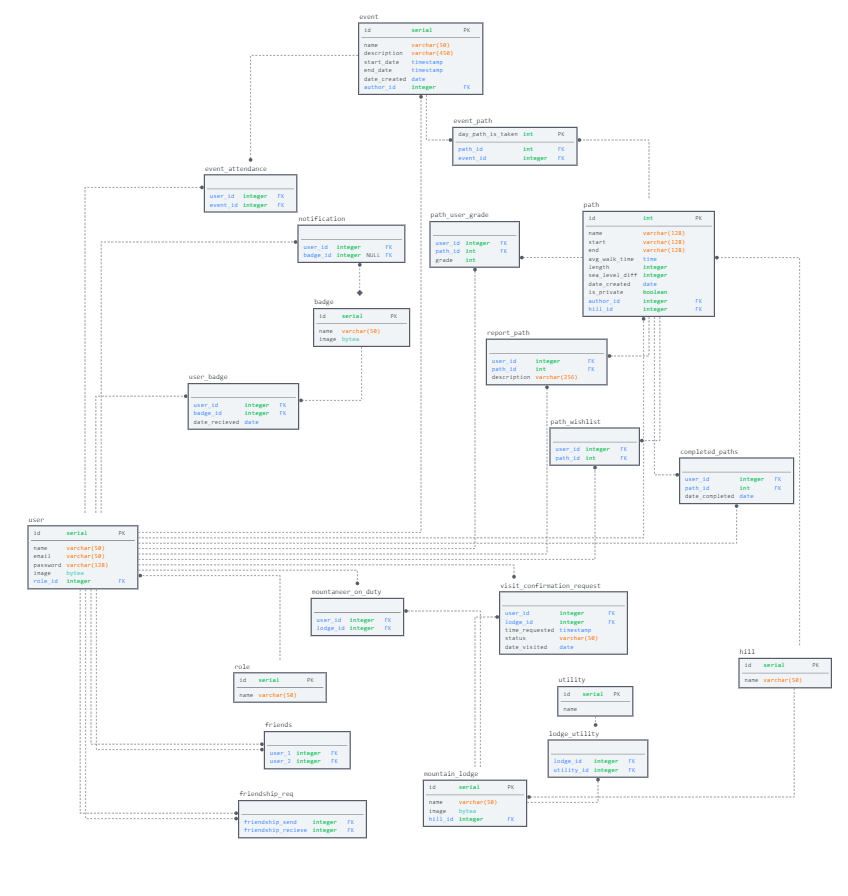
\includegraphics{slike/database.png}
			
			\eject
			
			
		\section{Dijagram razreda}
		
			\textit{Potrebno je priložiti dijagram razreda s pripadajućim opisom. Zbog preglednosti je moguće dijagram razlomiti na više njih, ali moraju biti grupirani prema sličnim razinama apstrakcije i srodnim funkcionalnostima.}\\
			
			\textbf{\textit{dio 1. revizije}}\\
			
			\textit{Prilikom prve predaje projekta, potrebno je priložiti potpuno razrađen dijagram razreda vezan uz \textbf{generičku funkcionalnost} sustava. Ostale funkcionalnosti trebaju biti idejno razrađene u dijagramu sa sljedećim komponentama: nazivi razreda, nazivi metoda i vrste pristupa metodama (npr. javni, zaštićeni), nazivi atributa razreda, veze i odnosi između razreda.}\\
			
			\textbf{\textit{dio 2. revizije}}\\			
			
			\textit{Prilikom druge predaje projekta dijagram razreda i opisi moraju odgovarati stvarnom stanju implementacije}
			
			
			
			\eject
		
		\section{Dijagram stanja}
			
			
			\textbf{\textit{dio 2. revizije}}\\
			
			\textit{Potrebno je priložiti dijagram stanja i opisati ga. Dovoljan je jedan dijagram stanja koji prikazuje \textbf{značajan dio funkcionalnosti} sustava. Na primjer, stanja korisničkog sučelja i tijek korištenja neke ključne funkcionalnosti jesu značajan dio sustava, a registracija i prijava nisu. }
			
			
			\eject 
		
		\section{Dijagram aktivnosti}
			
			\textbf{\textit{dio 2. revizije}}\\
			
			 \textit{Potrebno je priložiti dijagram aktivnosti s pripadajućim opisom. Dijagram aktivnosti treba prikazivati značajan dio sustava.}
			
			\eject
		\section{Dijagram komponenti}
		
			\textbf{\textit{dio 2. revizije}}\\
		
			 \textit{Potrebno je priložiti dijagram komponenti s pripadajućim opisom. Dijagram komponenti treba prikazivati strukturu cijele aplikacije.}